\documentclass{ctexart}
\usepackage{graphicx}
\usepackage{amsmath}
\usepackage{booktabs}
\usepackage[left=2.5cm,right=2.5cm,top=2.5cm,bottom=2.5cm]{geometry}
\begin{document}
\begin{center}
    \LARGE{电路实验第二课 预习报告}
\end{center}
\begin{center}
    Leo
\end{center}
\section{实验要求}
\begin{enumerate}
    \item 了解实验箱与面包板的结构和使用方法
    \item 了解电流表和电压表的结构以及内接和外接两种测量方法,分析其误差
    \item 使用数字万用表测量不同电阻的伏安特性
    \item 测量电容、电感的伏安特性
    \item 了解二极管结构,测量其伏安特性
\end{enumerate}
\section{实验原理(预习作业题)}
\subsection{面包板的用途与结构}
用途:面包板可以用于搭建小型的电路,免去了焊接操作,方便操作和调试。

结构:如图\ref{面包板示意图}所示,一块面包板可以分为三个部分:
\begin{enumerate}
    \item 上端每五个插孔横向成组,每组插孔相连
    \item 中间每五个插孔竖向成组,每组插孔相连
    \item 中间的凹槽起隔离作用
\end{enumerate}
\begin{figure}[ht]\label{面包板示意图}

    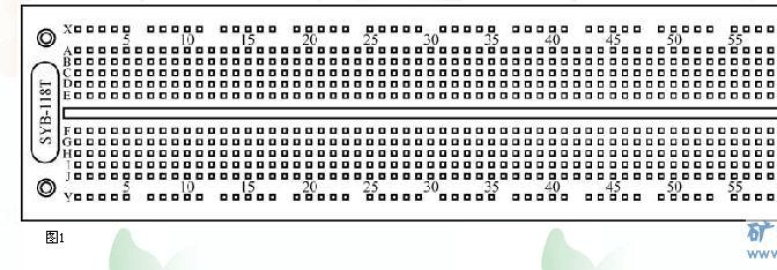
\includegraphics[scale=0.4]{./pictures/breadboard.jpeg}
    \caption{面包板示意图}
    
\end{figure}
\subsection{电阻的作用与识别方法}
电阻的作用非常广泛,最常见的有分压、分流、保护电路和滤波等等。

金属膜电阻一般用色环表示。色环电阻又分为四环和五环两种。两种都以环较为密集的一边为左边。四环电阻从左到右四个环分别为十位、个位、放大倍数、误差范围;五环电阻从左到右为百位、十位、个位、倍数、误差范围。

课上所发的电阻有:
\begin{table}[!ht]
    \centering
    \caption{课上所发电阻的参数}
    %\setlength{\tabcolsep}{20mm}%7可随机设置,调整到适合自己的大小为止
\begin{tabular}{cccc}
    \toprule[1.5pt]
    色环组合 & 阻值大小 & 误差范围 & 个数\\
    \midrule
    棕、黑、黑、金、棕  &10$\Omega$ &[F]$\pm1\%$ &2\\
    棕、棕、黑、黑、棕  &110$\Omega$  &[F]$\pm1\%$  & 2\\
    棕、黑、黑、黑、棕  &100$\Omega$ &[F]$\pm1\%$ &2\\
    红、黑、黑、黄、棕  &2000k$\Omega$ &[F]$\pm1\%$  &1\\
    红、黑、黑、红、棕  &200k$\Omega$  &[F]$\pm1\%$ & 2\\
    棕、黑、黑、红、棕  &10k$\Omega$ &[F]$\pm1\%$&3\\
    红、黑、黑、棕、棕  &2k$\Omega$&[F]$\pm1\%$ &2\\
    \bottomrule
    \end{tabular}
\end{table}


\subsection{了解电容}
独石电容(MLC)是一种一种多层叠片烧结成整体独石结构的陶瓷电容器,具有体积小、电容量大、绝缘电阻、耐温性能好等特点。其外形如图所示
\begin{figure}[!ht]\label{独石电容}
    \centering 
    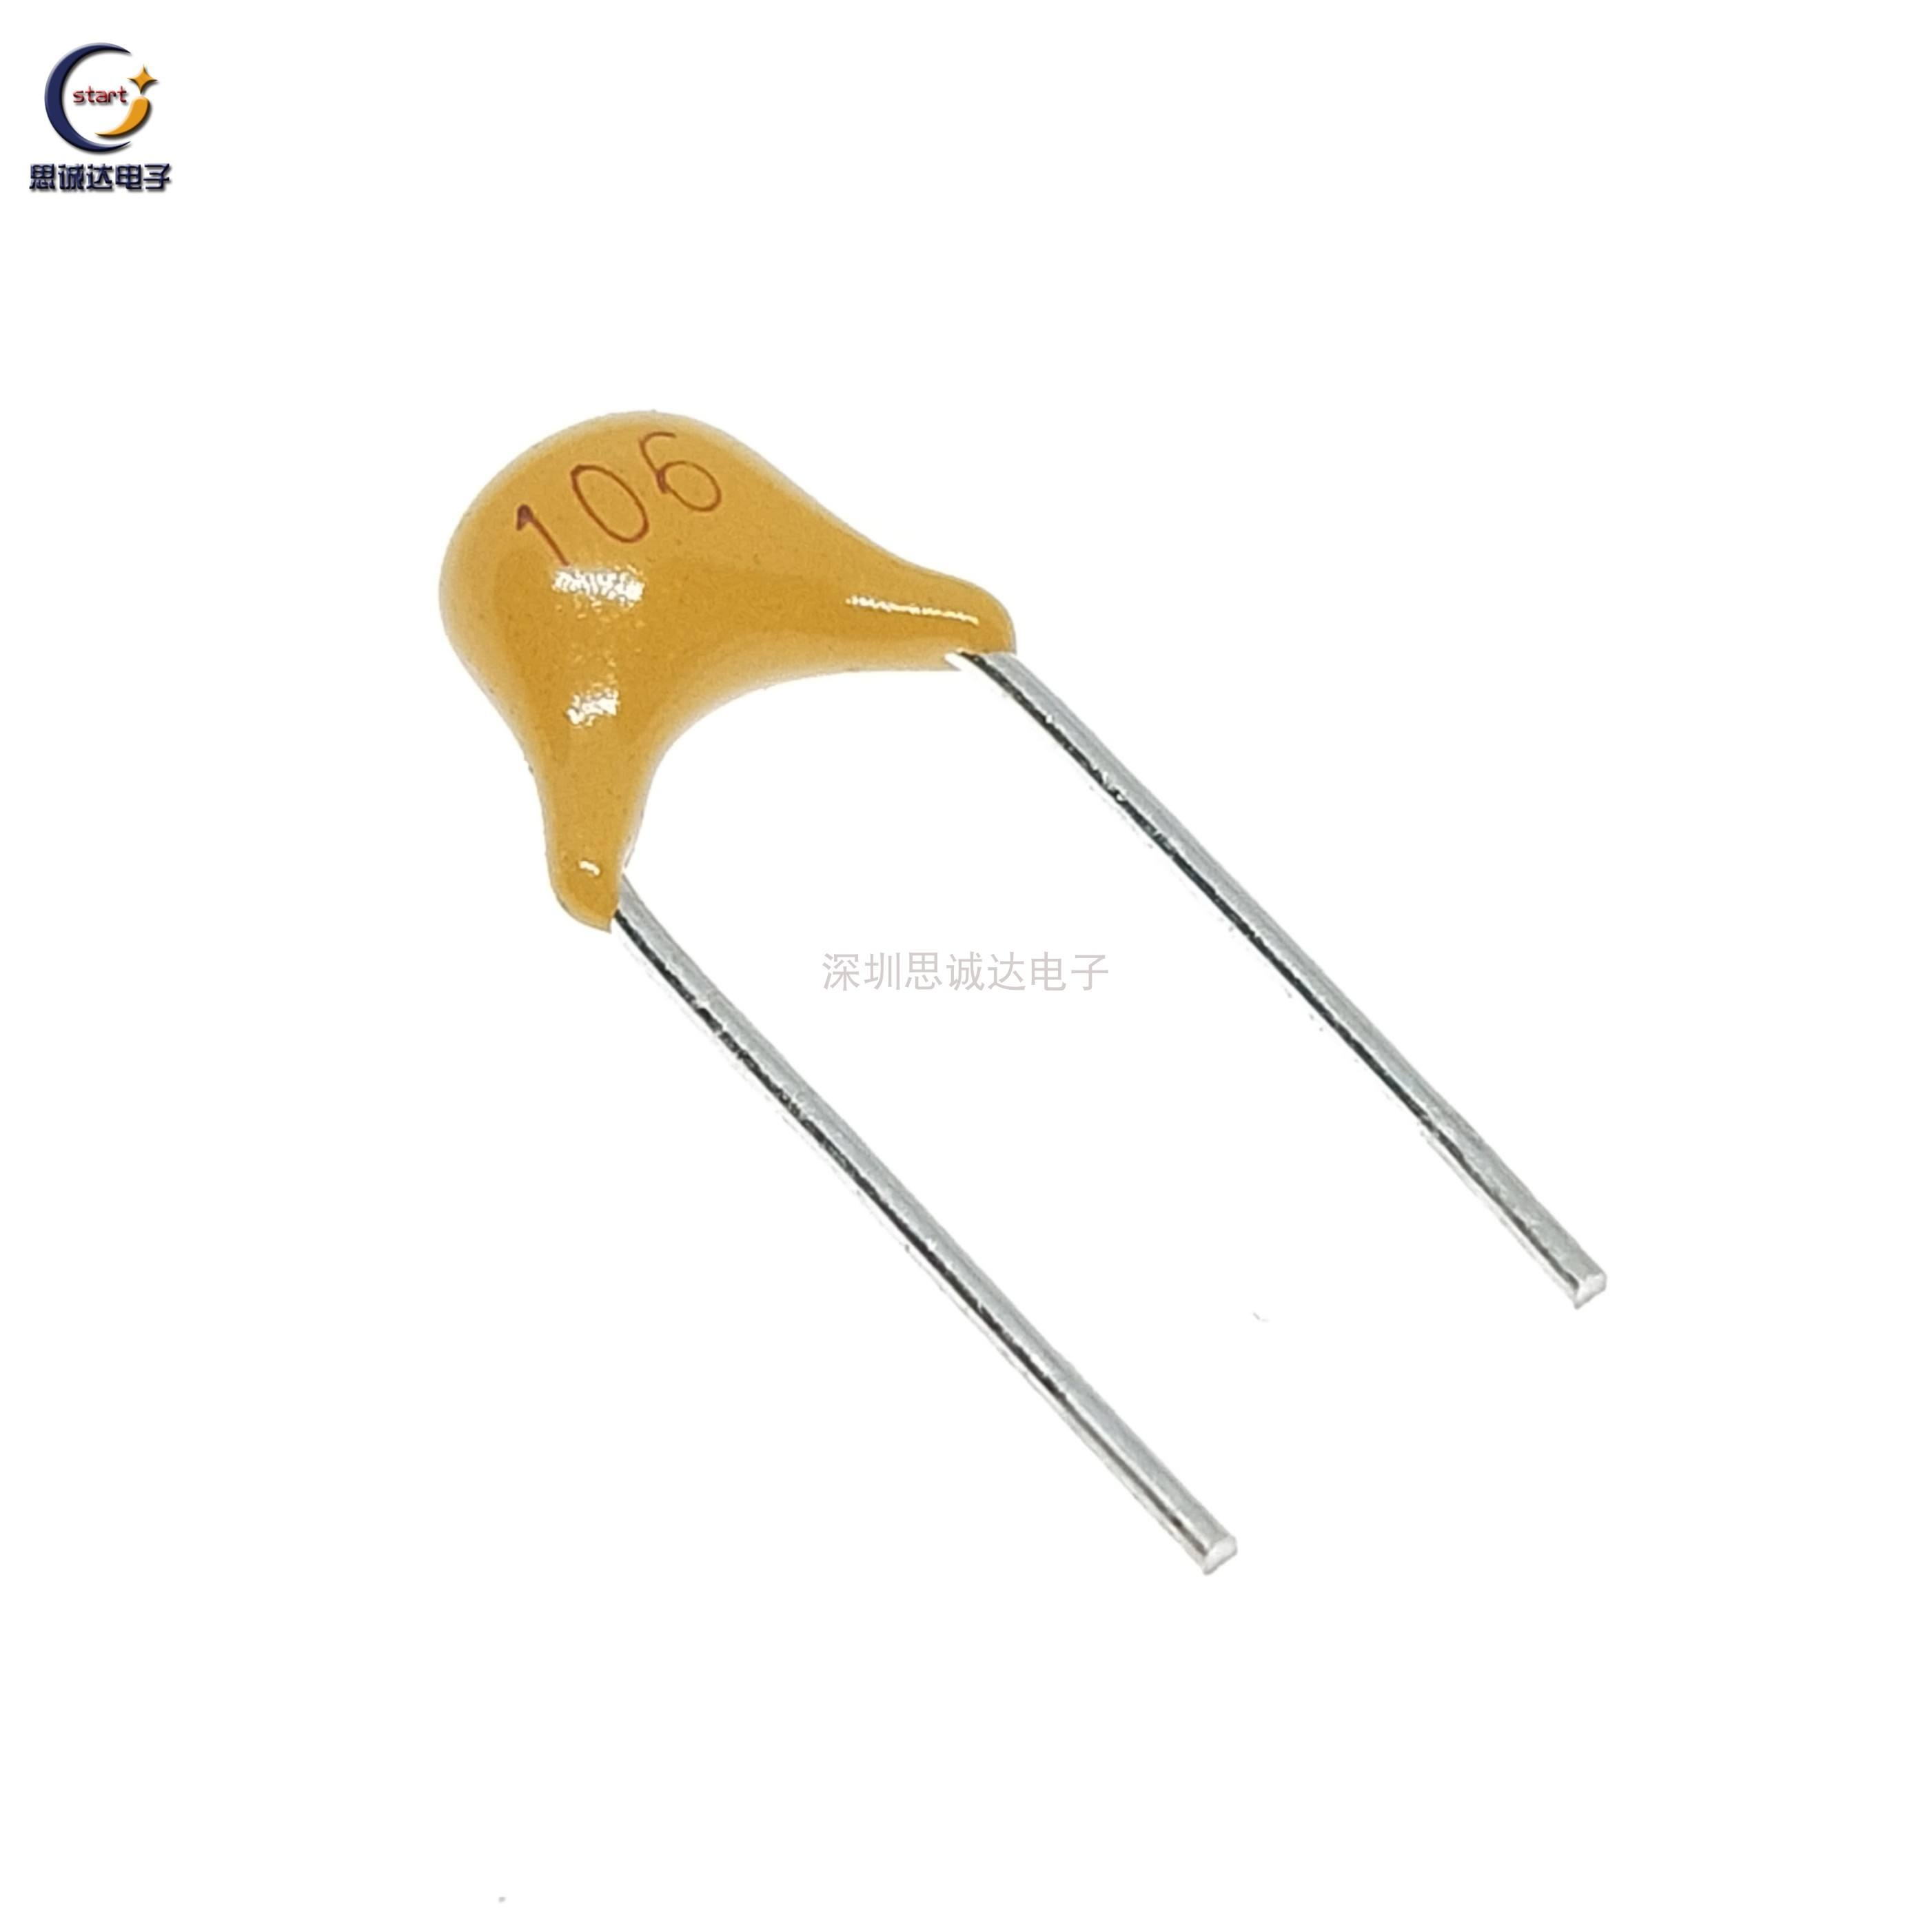
\includegraphics[scale=0.06]{./pictures/独石电容.jpeg}
    \caption{独石电容}  
\end{figure}
电容量的读取:独石电容上面有容量数字标称,前两位表示有效值,后一位表示倍率,单位为pF。,比如103,就是$10\times 10^3$pF。

电容器的耐压:查阅资料得本课所涉及的103独石电容耐压均为100V。
\subsection{了解二极管}
所发的三个二极管均为C6V2型号,属于稳压管,对应的参数为
\begin{enumerate}
    \item Zener Voltage Range Vznom稳定电压:6.2V
    \item Zener Voltage Range lZT稳定电流 :5mA
    
    \item Dynamic Resistance rZJT最小动态电阻 :10Ω
    
    \item Dynamic Resistance rZJK最大动态电阻 :200Ω
    
    \item Reverse Leakage Current反向漏电流 :2μA
\end{enumerate}



\subsection{电流表和电压表的结构与使用}
UT803型万用表的电流表内阻一般为10Ω,电压表内阻一般为10MΩ。至于交流电压表,适用的频率范围通常为45Hz到1000Hz。

电流表:电流计与小电阻串联。电压表:电流计和大电阻并联。

内接法:电流表直接测量的是待测电阻的电流,电压表测得的是电流表和待测电阻共同的电压。结果:电流测量准确,电压偏大,所以电阻测量值偏大。适用于大电阻的测量,因为此时电流表的分压影响不明显。

外接法:电流表测得流过电压表和电阻的电流之和,电压表测得电阻上的电压。结果:电流偏大,电压准确,所以电阻测量值偏小。适用于小电阻的测量,因为此时电压表的分流作用不明显。
\begin{figure}[!ht]\label{电表的两种接法}
    \centering
    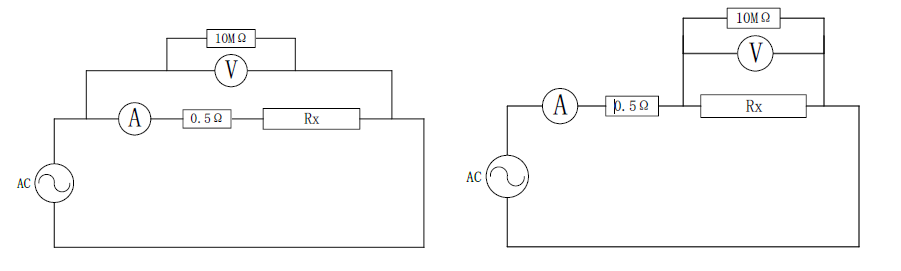
\includegraphics[scale=0.7]{./pictures/电流表的两种接法.png}
    \caption{电表的两种接法}
    
\end{figure}
\subsection{电容容抗、电感阻抗与频率的关系}
查阅资料得到电容容抗、电感阻抗的表达式:
\begin{equation}
    \begin{cases}
        X_C= \dfrac{1}{2 \pi f C}\\
        X_L = 2 \pi f L
    \end{cases}
\end{equation}
所以容抗和频率成反比,感抗和频率成正比。



\section{其他实验基础知识}\subsection{二极管的特性:单向导电性}
\subsubsection{伏安特性}
在二极管加有正向电压,当电压值较小时,电流极小;当电压超过某个阈值时,电流开始按指数规律增大,通常称此为二极管的开启电压;当电压达到更高的某个值时,二极管处于完全导通状态,通常称此电压为二极管的导通电压,用符号UD表示。
\subsubsection{正向电压}
外加正向电压时,在正向特性的起始部分,正向电压很小,正向电流几乎为零,这一段称为死区。这个不能使二极管导通的正向电压称为死区电压。 

当正向电压大于死区电压以后,二极管正向导通,电流随电压增大而迅速上升。在正常使用的电流范围内,导通时二极管的端电压几乎维持不变,这个电压称为二极管的正向电压。
\subsubsection{反向电压}
当反向电压较小时,通过二极管的电流极小,可以近似为开路;但当反向电压大于某一个阈值后,反向电流急剧增加,称此时的二极管被反向击穿。
\begin{figure}[!ht]\label{二极管的伏安特性}
    \centering
    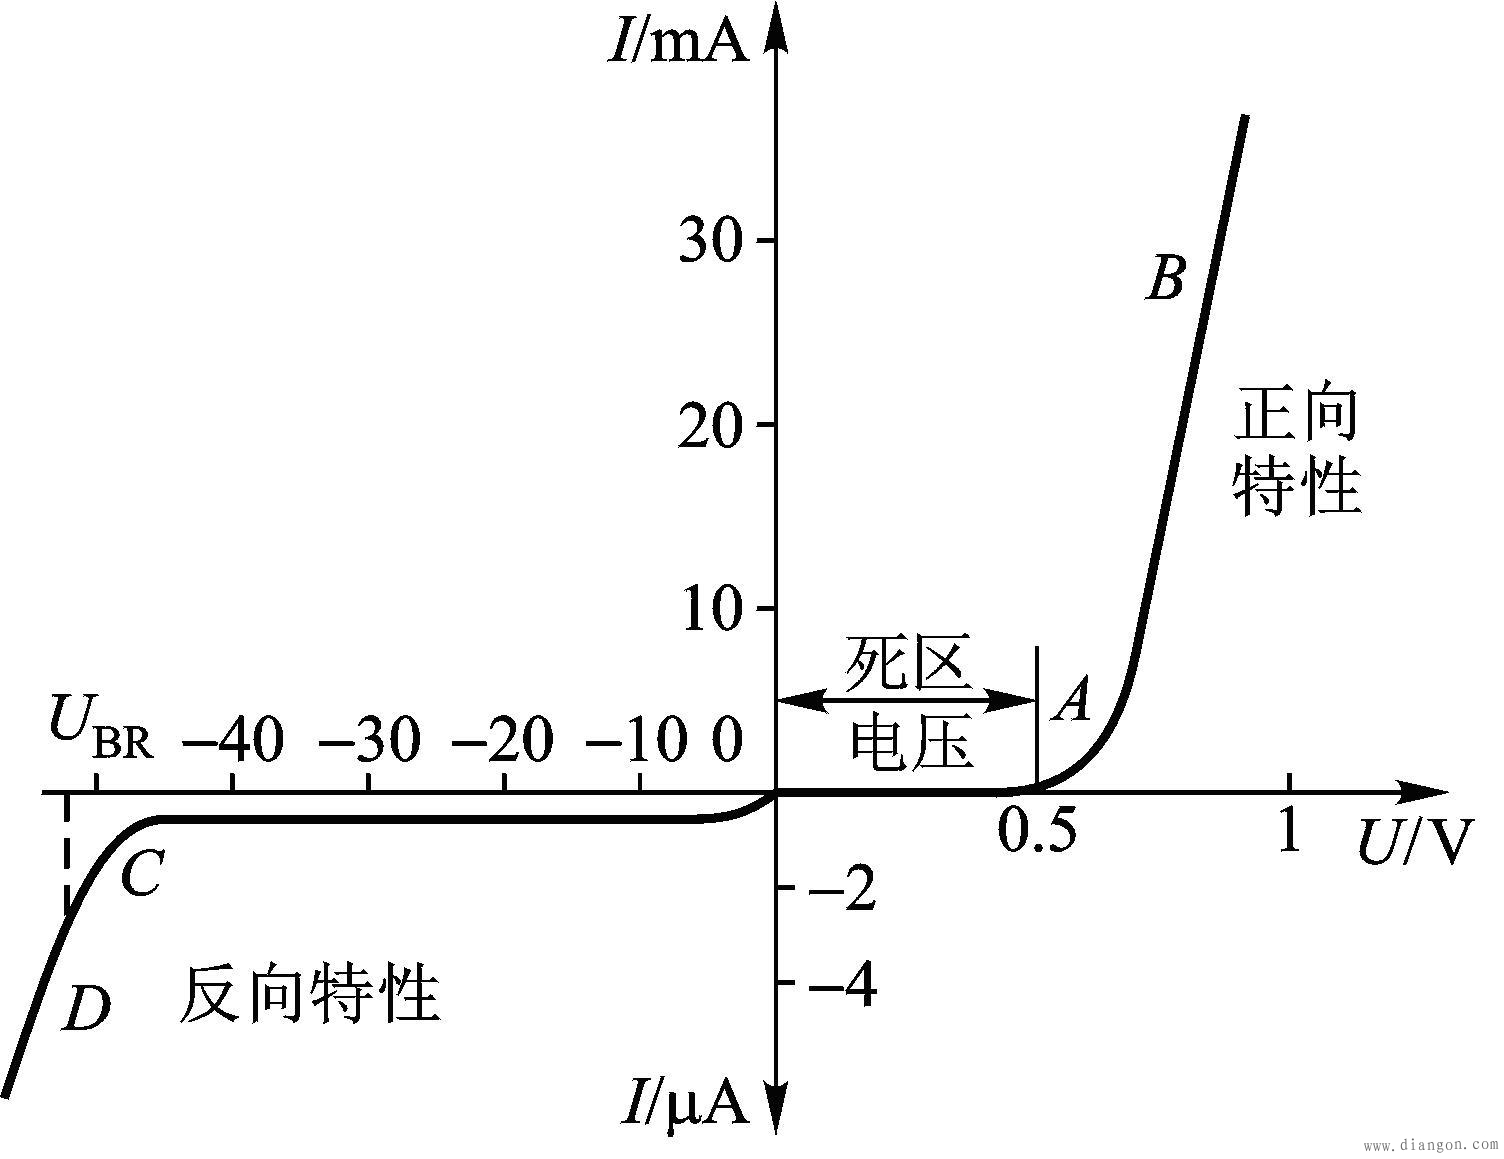
\includegraphics[scale=0.15]{./pictures/二极管伏安特性.jpg}
    \caption{二极管的伏安特性}
    
\end{figure}
\subsection{稳压管}
\subsubsection{稳压管的特性:稳定输出电压}
稳压管是一种特殊的二极管,这种二极管的死区范围很大。稳压管是一种直到临界击穿电压前都具有很高电阻的半导体器件。稳压管在反向击穿时,在一定的电流范围内(或者说在一定功率损耗范围内),端电压几乎不变,表现出稳压特性。
\subsubsection{稳压管伏安特性的测量}
首先搭建如图所示的电路,(稳压管正接),持续缓慢增大电压,当电压表示数不再明显增大时,记为稳压管的稳定电压。然后将其反接,同样的方法可以测得反向稳定电压。
\begin{figure}\label{稳压管伏安特性的测量}
    \centering
    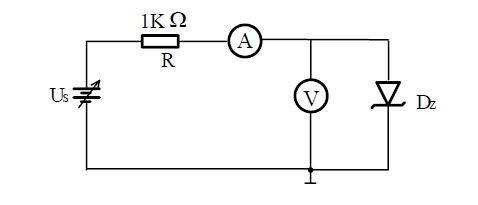
\includegraphics[scale=1.2]{./pictures/稳压管伏安特性的测量.png}
    \caption{稳压管伏安特性的测量}
\end{figure}


\end{document}